\documentclass[tikz,border=8pt]{standalone}
% Shared look for every TikZ diagram. Load with \input{../../tools/tikz-style.tex}
\usepackage[sfdefault]{roboto}
\usetikzlibrary{arrows.meta, positioning, shapes.geometric, calc, fit, backgrounds}
\definecolor{cblue}{HTML}{4C78A8}
\definecolor{corange}{HTML}{F58518}
\definecolor{cgreen}{HTML}{54A24B}
\definecolor{cred}{HTML}{E45756}
\definecolor{cpurple}{HTML}{B279A2}
\definecolor{cgrey}{HTML}{6B6B6B}
\tikzset{
  every picture/.style={font=\sffamily, line width=1.2pt},
  box/.style={draw=#1, fill=#1!12, rounded corners=4pt, align=center, inner sep=7pt, minimum height=1.1cm},
  box/.default=cgrey,
  arrow/.style={-{Stealth[length=3mm]}, draw=cgrey, line width=1.4pt},
  title/.style={font=\sffamily\bfseries\Large},
  note/.style={font=\sffamily\small, text=cgrey, align=center},
}
\AtBeginDocument{\hyphenpenalty=10000 \exhyphenpenalty=10000}

% The four layers in three real stacks, with their rates read from the code (2026-10-12):
% Nav2 (ros-navigation/navigation2, main): nav2_bringup/params/nav2_params.yaml (bt_loop_duration 10 ms;
%   global_costmap update_frequency 1.0; local_costmap update_frequency 5.0; controller_frequency 20.0;
%   velocity_smoother smoothing_frequency 20.0) and the default tree navigate_to_pose_w_replanning_and_recovery.xml
%   (RateController hz 1.0 around ComputePathToPose).
% Autoware (autowarefoundation/autoware_launch, main): behavior_path_planner.param.yaml planning_hz 10.0;
%   trajectory_follower_node.param.yaml ctrl_period 0.03.
% Apollo (ApolloAuto/apollo, master): planning_gflags.cc planning_loop_rate 10; control.dag interval 10 (ms).
\begin{document}
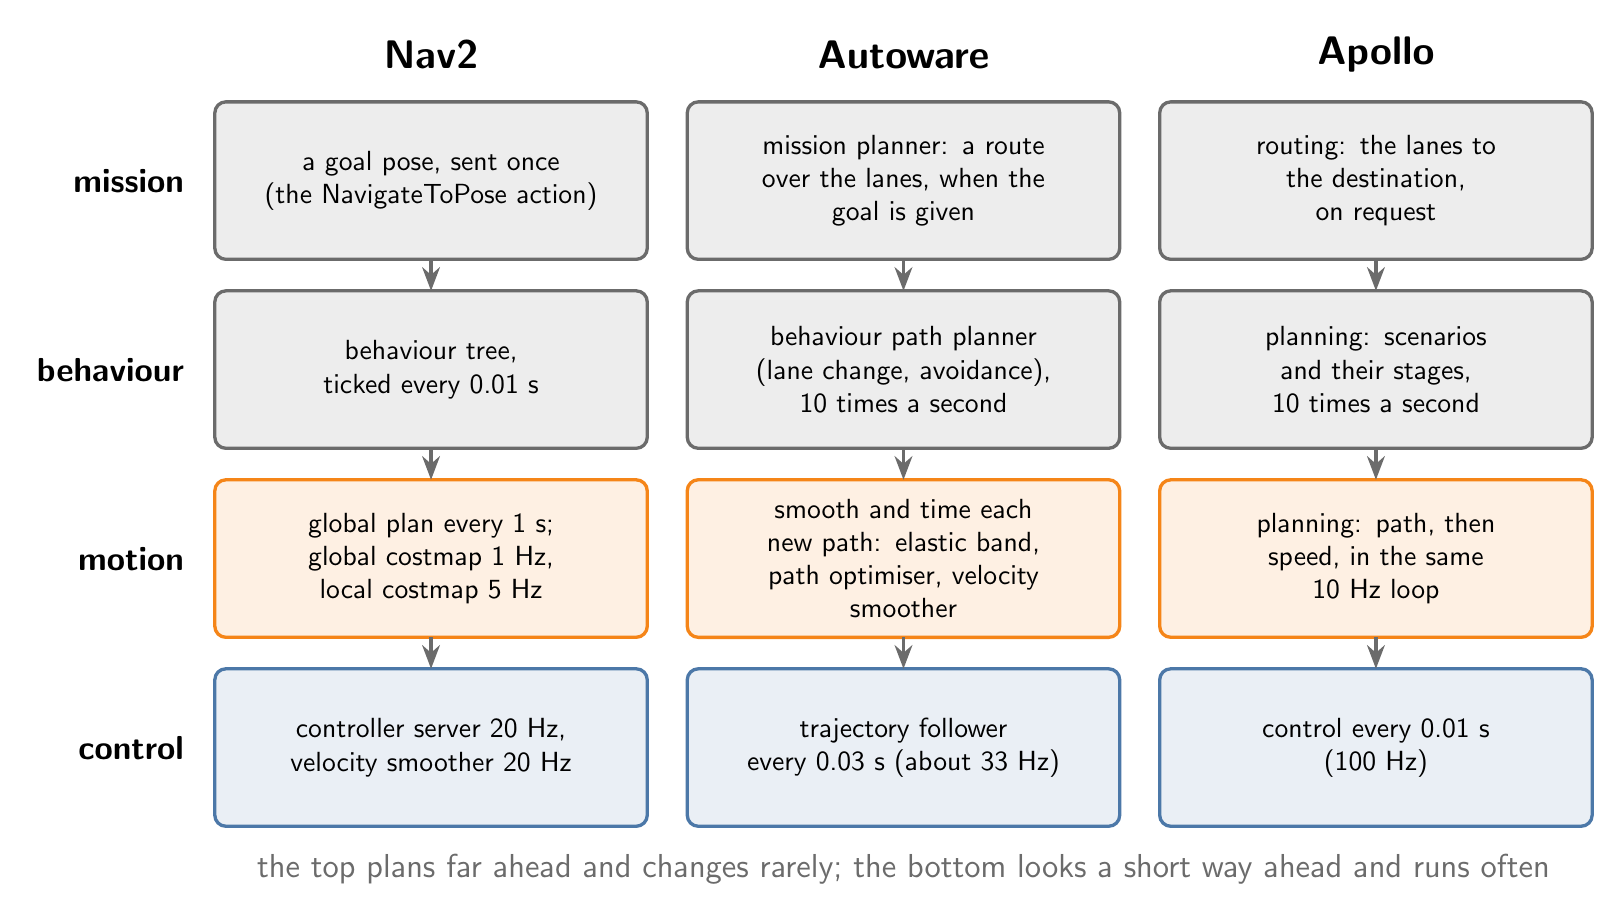
\begin{tikzpicture}[
  c/.style={box=#1, minimum width=5.3cm, text width=5.0cm, minimum height=2.0cm, font=\sffamily},
  lab/.style={font=\sffamily\bfseries\large, align=right, anchor=east}]
  \foreach \name/\x in {Nav2/0, Autoware/6, Apollo/12} \node[title] at (\x,1.6) {\name};
  \foreach \lay/\y in {mission/0, behaviour/-2.4, motion/-4.8, control/-7.2} \node[lab] at (-3.0,\y) {\lay};
  % Nav2
  \node[c=cgrey] at (0,0) {a goal pose, sent once\\ (the NavigateToPose action)};
  \node[c=cgrey] at (0,-2.4) {behaviour tree,\\ ticked every 0.01 s};
  \node[c=corange] at (0,-4.8) {global plan every 1 s;\\ global costmap 1 Hz,\\ local costmap 5 Hz};
  \node[c=cblue] at (0,-7.2) {controller server 20 Hz,\\ velocity smoother 20 Hz};
  % Autoware
  \node[c=cgrey] at (6,0) {mission planner: a route\\ over the lanes, when the\\ goal is given};
  \node[c=cgrey] at (6,-2.4) {behaviour path planner\\ (lane change, avoidance),\\ 10 times a second};
  \node[c=corange] at (6,-4.8) {smooth and time each\\ new path: elastic band,\\ path optimiser, velocity\\ smoother};
  \node[c=cblue] at (6,-7.2) {trajectory follower\\ every 0.03 s (about 33 Hz)};
  % Apollo
  \node[c=cgrey] at (12,0) {routing: the lanes to\\ the destination,\\ on request};
  \node[c=cgrey] at (12,-2.4) {planning: scenarios\\ and their stages,\\ 10 times a second};
  \node[c=corange] at (12,-4.8) {planning: path, then\\ speed, in the same\\ 10 Hz loop};
  \node[c=cblue] at (12,-7.2) {control every 0.01 s\\ (100 Hz)};
  \foreach \x in {0,6,12} {
    \draw[arrow] (\x,-1.0) -- (\x,-1.4); \draw[arrow] (\x,-3.4) -- (\x,-3.8); \draw[arrow] (\x,-5.8) -- (\x,-6.2); }
  \node[note, font=\sffamily\large] at (6,-8.75) {the top plans far ahead and changes rarely; the bottom looks a short way ahead and runs often};
\end{tikzpicture}
\end{document}
